% ============================================================
% IE500 Data Mining -- Team 9 Brewed Clusters -- Project Report
% Compiled with: pdflatex main.tex  (run twice for TOC)
% NOTE: Replace this preamble with the official DWS thesis
%       LaTeX template before final submission.
% ============================================================
\documentclass[11pt, a4paper]{article}

\usepackage[top=2.5cm, bottom=2.5cm, left=2.5cm, right=2.5cm]{geometry}
\usepackage[utf8]{inputenc}
\usepackage[T1]{fontenc}
\usepackage{lmodern}
\usepackage{microtype}
\usepackage{graphicx}
\usepackage{booktabs}
\usepackage{tabularx}
\usepackage{multirow}
\usepackage{amsmath}
\usepackage{xcolor}
\usepackage{colortbl}
\usepackage[colorlinks=true, linkcolor=black, citecolor=black, urlcolor=blue!60!black]{hyperref}
\usepackage{float}
\usepackage{caption}
\usepackage{subcaption}
\usepackage{enumitem}
\usepackage{parskip}
\usepackage{array}
\usepackage{makecell}
\usepackage{authblk}

\setlength{\parskip}{4pt}
\setlength{\parindent}{0pt}
\captionsetup{font=small, labelfont=bf, skip=4pt}
\setlist[itemize]{noitemsep, topsep=2pt}

% ── Colour helpers ──────────────────────────────────────────
\definecolor{lightgrey}{RGB}{242,242,242}
\definecolor{darkblue}{RGB}{31,56,100}
\newcommand{\hdr}[1]{\cellcolor{darkblue}\textcolor{white}{\textbf{#1}}}
\newcommand{\rowgrey}{\rowcolor{lightgrey}}

% ── Short-hands ─────────────────────────────────────────────
\newcommand{\ttf}[1]{\texttt{#1}}
\newcommand{\mf}[1]{$\text{#1}$}

% ============================================================
\begin{document}

% ── Title page ───────────────────────────────────────────────
\begin{titlepage}
  \centering
  \vspace*{1.5cm}
  {\Large\bfseries University of Mannheim\\[0.3em]
   Data and Web Science Group\\[0.3em]
   IE500 Data Mining\par}
  \vspace{2cm}
  {\LARGE\bfseries Predicting Game Success on the\\[0.4em]
   Steam Platform\par}
  \vspace{0.8cm}
  {\large Multiclass Classification of Steam Game Reception\par}
  \vspace{2cm}
  {\large\bfseries Team 9 -- Brewed Clusters\par}
  \vspace{0.6cm}
  \begin{tabular}{l}
    Satwik Kumar Lohani      \\
    Arpitha Shivaprasad Kori \\
    Zubair Ashfaq            \\
    Beyza \"{U}nl\"{u}       \\
    Muhammad Sameer Siddiqui \\
    Esha Raheel              \\
  \end{tabular}
  \vspace{2cm}

  {\large Spring Semester 2026\par}
  \vspace{0.5cm}
  {\normalsize Submitted to the Data and Web Science Group,
               University of Mannheim\par}
  \vfill
  {\small\textit{AI-assisted tools (Claude Code by Anthropic) were used
  for code generation, LaTeX drafting, and report editing.
  All analytical decisions, model training, and result interpretation
  were performed and verified by the team.}}
\end{titlepage}

% ── Table of contents ────────────────────────────────────────
\tableofcontents
\newpage

% ============================================================
\section{Introduction and Application Area}
\label{sec:intro}

The Steam marketplace hosts over 50,000 active titles, making game reception an important
signal for developers and publishers. This project builds a multiclass classification pipeline
to predict whether a Steam game will receive predominantly positive (\textit{Good}),
mixed (\textit{Mixed}), or negative (\textit{Bad}) reviews, using only metadata available at
or near release time.

Beyond predictive accuracy, we aim to identify which game attributes most strongly drive
positive reception -- providing actionable insight for developers making design, pricing,
and platform decisions.

The task is non-trivial: reception is determined by an interaction of content type,
community tags, pricing, and platform availability -- a high-dimensional signal that
linear intuition does not capture well.
The primary evaluation metric is \textbf{Macro F1-score}, which weights all three
classes equally regardless of their frequency in the data.

% ============================================================
\section{Dataset Profile}
\label{sec:data}

\subsection{Source and size}
The dataset is the \textit{Steam Games Dataset} from Kaggle
(FronkonGames, 2024) \cite{fronkon2024}, retrieved via the Steam API and SteamSpy.
The raw CSV contains 122,611 rows and 39 columns covering game metadata
(price, genres, tags, categories, platform flags, DLC count, achievements, etc.).

\begin{table}[H]
  \centering\small
  \caption{Dataset pipeline summary.}
  \label{tab:datapipeline}
  \begin{tabularx}{\linewidth}{lrrl}
    \toprule
    \textbf{Stage} & \textbf{Rows} & \textbf{Columns} & \textbf{Action} \\
    \midrule
    Raw CSV              & 122,611 & 39 & CSV row-alignment fix; drop URL/media columns \\
    After weak-col drop  & 122,611 & 28 & Retained modeling-relevant columns \\
    After review filter  &  56,655 & 28 & Removed games with $<10$ total reviews \\
    Train split (80\,\%) &  45,324 & 147 & Stratified split; StandardScaler on numerics \\
    Test split  (20\,\%) &  11,331 & 147 & Held out until final evaluation \\
    \bottomrule
  \end{tabularx}
\end{table}

\subsection{Target construction}
A multiclass label was derived from the review ratio
$r = \text{Positive} / (\text{Positive} + \text{Negative})$.
Two threshold schemes were compared empirically
(detailed in Section~\ref{sec:threshold}); the \textbf{0.50 threshold} was
selected as the project standard.

\begin{table}[H]
  \centering\small
  \caption{Selected threshold scheme and resulting class distribution (train split).}
  \label{tab:classdist}
  \begin{tabular}{lccr}
    \toprule
    \textbf{Class} & \textbf{Rule} & \textbf{Train count} & \textbf{Share} \\
    \midrule
    Good  & $r \geq 0.75$          & 28,671 & 63.3\,\% \\
    Mixed & $0.50 \leq r < 0.75$   & 12,834 & 28.3\,\% \\
    Bad   & $r < 0.50$             &  3,819 &  8.4\,\% \\
    \bottomrule
  \end{tabular}
\end{table}

\subsection{Feature space}
The safe feature set (147 columns) excludes post-release variables
(\ttf{avg\_playtime}, \ttf{Recommendations}, \ttf{Metacritic score})
that would constitute data leakage.

\begin{table}[H]
  \centering\small
  \caption{Feature groups in the 147-column safe training set.}
  \label{tab:features}
  \begin{tabular}{llr}
    \toprule
    \textbf{Group}   & \textbf{Examples} & \textbf{Count} \\
    \midrule
    Numeric metadata & \ttf{log\_price}, Achievements, \ttf{n\_languages}, DLC count & 5 \\
    Platform flags   & Windows, Mac, Linux & 3 \\
    Release era      & \ttf{era\_pre-2015}, \ttf{era\_2015-2019}, \ttf{era\_2020+} & 3 \\
    Genres           & Action, Indie, RPG, \ldots & 28 \\
    Categories       & Single-player, Co-op, Steam Cloud, \ldots & 58 \\
    Tags (top 50)    & Singleplayer, 2D, Casual, \ldots & 50 \\
    \midrule
    \textbf{Total}   & & \textbf{147} \\
    \bottomrule
  \end{tabular}
\end{table}

Most features are sparse binary indicators.
This is an important constraint: the project has many features but individually limited
discriminative power, which contributes to the observed performance ceiling.

% ============================================================
\section{Preprocessing}
\label{sec:preprocessing}

The preprocessing pipeline was applied identically to both threshold versions of the dataset.

\begin{itemize}
  \item \textbf{Duplicate and validity checks.} Exact-duplicate rows were identified
        and removed (fewer than 0.1\,\% of records).
        Numeric columns were validated for range plausibility
        (e.g.\ negative prices or review counts set to zero were flagged and corrected).
  \item \textbf{Row-alignment fix.} The raw CSV had misaligned rows caused by unparsed
        text fields; corrected before any downstream processing.
  \item \textbf{Numeric conversion.} Peak CCU, Positive, Negative, Price, Achievements,
        playtime, Recommendations, and Metacritic score were cast to numeric types.
  \item \textbf{Weak-column removal.} AppID, screenshot URLs, header image, website,
        review text, and support links were removed.
  \item \textbf{Review-stability filter.} Games with fewer than 10 total reviews were
        excluded (122,611 $\to$ 56,655 rows) to avoid unstable labels.
  \item \textbf{Multi-value parsing.} Genre, Category, and Tag fields (comma-separated
        strings) were binarised using \texttt{MultiLabelBinarizer}; the top 50 tags by
        training-set frequency were retained.
  \item \textbf{Derived features.} \texttt{log\_price} (log-transform to reduce right
        skew), release era buckets (\texttt{pre-2015 / 2015-2019 / 2020+}),
        and \texttt{n\_languages} (count of supported languages).
  \item \textbf{Leakage-aware split.} Post-release engagement signals
        (\texttt{avg\_playtime}, \texttt{Recommendations}, \texttt{Metacritic})
        were excluded from the safe feature set used for all modeling.
  \item \textbf{Scaling.} \texttt{StandardScaler} was fitted on the training split only
        and applied to all continuous safe features.
  \item \textbf{Outlier treatment.} A robustness check capping
        \texttt{Achievements} and \texttt{n\_languages} at the 99th percentile
        (train-only) showed no improvement in Macro F1; explicit capping was not adopted.
\end{itemize}

% ============================================================
\section{Exploratory Data Analysis}
\label{sec:eda}

EDA on the safe training set revealed four modelling-relevant patterns.
(1) \textbf{Class imbalance}: Good (63.3\,\%) dominates; Bad (8.4\,\%) is the minority.
(2) \textbf{Sparse features}: most binary indicators are True for fewer than 20\,\% of
games, so individual features have limited separating power.
(3) \textbf{Weak numeric correlations}: simple Pearson correlations between safe numeric
features and a Good-vs-rest indicator are all below $|0.15|$, confirming the task
requires non-linear combination.
(4) \textbf{Descriptor patterns}: categories linked to accessibility
(\texttt{cat\_Steam Cloud}, \texttt{cat\_Full controller support}) and the recent release
era (\texttt{era\_2020+}) show descriptively higher good-reception rates;
monetisation-heavy categories trend lower. These were treated as descriptive patterns,
not causal claims.

% ============================================================
\section{Modelling}
\label{sec:modelling}

\subsection{Setup}
All models were evaluated using \textbf{nested cross-validation}:
5 outer folds for unbiased performance estimation and 3 inner folds for
\texttt{GridSearchCV} hyperparameter selection.
The primary metric throughout is \textbf{Macro F1}, which penalises poor minority-class
performance equally with majority-class errors.
Class imbalance was handled via \texttt{class\_weight=`balanced'} (or equivalent)
inside each model's pipeline.

\subsection{Models trained}
Seven models were trained and compared
(Table~\ref{tab:models}).
A majority-class classifier (always predicts \textit{Good}) gives Macro F1 $\approx 0.26$
(Good F1 = 0.775, Mixed = Bad = 0) and serves as the lower bound.

\begin{table}[H]
  \centering\small
  \caption{Full model comparison on the 0.50-threshold dataset (147 safe features).}
  \label{tab:models}
  \begin{tabularx}{\linewidth}{Xrrrrrrl}
    \toprule
    \textbf{Model} & \textbf{CV F1} & \textbf{Std} & \textbf{Test F1} &
    \textbf{Good} & \textbf{Mixed} & \textbf{Bad} & \textbf{Best params} \\
    \midrule
    \rowcolor{green!15}
    Random Forest        & 0.5093 & 0.0073 & \textbf{0.5100} & 0.77 & 0.43 & 0.33 &
      depth=None, leaf=4, est=200 \\
    XGBoost              & 0.4820 & 0.0039 & 0.4799 & 0.73 & 0.39 & 0.31 &
      lr=0.1, depth=6, est=200 \\
    Linear SVM           & 0.4680 & 0.0034 & 0.4693 & 0.77 & 0.34 & 0.29 &
      C=0.1, balanced \\
    LR + SMOTE           & 0.4619 & 0.0064 & 0.4648 & 0.73 & 0.39 & 0.27 &
      C=0.1 \\
    KNN                  & 0.4462 & 0.0066 & 0.4516 & 0.77 & 0.38 & 0.21 &
      k=11, Manhattan, distance \\
    LR baseline          & 0.4385 & 0.0034 & 0.4355 & 0.70 & 0.33 & 0.28 &
      C=0.1, L2 \\
    LR + ROS             & 0.4376 & 0.0038 & 0.4352 & 0.70 & 0.33 & 0.28 &
      C=0.01 \\
    \midrule
    Majority class (Good)& ---    & ---    & 0.2583 & 0.78 & 0.00 & 0.00 &
      always predict Good \\
    \bottomrule
  \end{tabularx}
\end{table}

\begin{figure}[H]
  \centering
  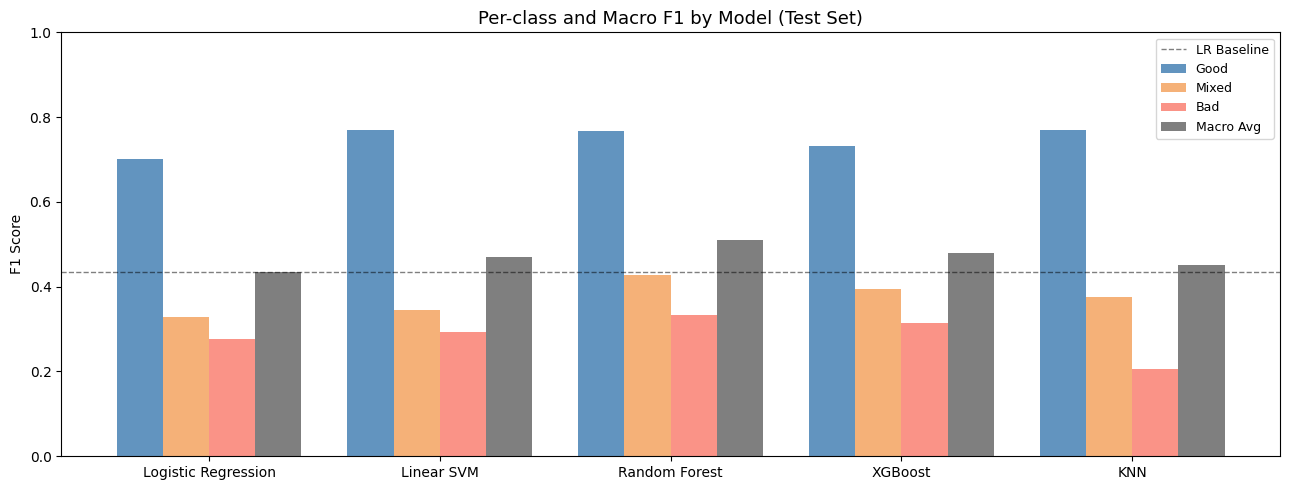
\includegraphics[width=0.92\linewidth]{figures/fig03_model_comparison.png}
  \caption{Per-class F1 comparison across all models on the test set.}
  \label{fig:model_comparison}
\end{figure}

\subsection{Key modelling findings}

\textbf{Random Forest} (Test Macro F1 = 0.5100) is the best overall model.
Tree-based methods (RF, XGBoost) outperform linear ones (SVM, LR) because the feature
space contains many overlapping binary indicators whose interactions are non-linear.
RF achieves the best balance across all three classes; XGBoost recovers higher Bad recall
(0.56) but lower Good F1, resulting in second rank.

\textbf{KNN} beats the LR baseline (+0.016) but has the lowest Bad F1 (0.21) due to
the absence of class-weight support in the standard scikit-learn implementation.
A 15,000-sample stratified subsample was required for tractable training.

\subsection{Imbalance handling (LR comparison)}

\begin{table}[H]
  \centering\small
  \caption{Imbalance handling strategies on Logistic Regression.}
  \label{tab:imbalance}
  \begin{tabular}{lrrrrrr}
    \toprule
    \textbf{Strategy} & \textbf{CV F1} & \textbf{Test F1} &
    \textbf{Good} & \textbf{Mixed} & \textbf{Bad} & \textbf{vs Baseline} \\
    \midrule
    LR + SMOTE           & 0.4619 & 0.4648 & 0.73 & 0.39 & 0.27 & $+$0.0293 \\
    LR + class\_weight   & 0.4385 & 0.4355 & 0.70 & 0.33 & 0.28 & baseline  \\
    LR + ROS             & 0.4376 & 0.4352 & 0.70 & 0.33 & 0.28 & $-$0.0003 \\
    \bottomrule
  \end{tabular}
\end{table}

SMOTE (+0.029) is the only strategy that provides a meaningful gain; it creates
synthetic minority samples via interpolation, giving the model genuinely new patterns.
ROS (random duplication) adds no information and matches the baseline.

\subsection{Symbolic model interpretation: Logistic Regression}
\label{sec:lr_interp}

Logistic Regression (LR) is the interpretable symbolic baseline.
With L2 regularisation (C\,=\,0.1) and \texttt{class\_weight=`balanced'}, it learns a
linear decision boundary in the 147-feature space -- making its coefficients directly
readable as feature contributions.

Inspecting the LR coefficients for the \textit{Good} class (multinomial one-vs-rest)
shows a pattern consistent with the feature-separation analysis (Section~\ref{sec:evaluation}):
\begin{itemize}
  \item \textbf{Strongest positive predictors (Good):}
        \ttf{era\_2020+}, \ttf{cat\_Steam Cloud}, \ttf{tag\_2D},
        \ttf{tag\_Singleplayer}, \ttf{cat\_Full controller support}.
        These align with the top Good$-$Mixed feature differences ($+$0.13 to $+$0.17),
        confirming that modern, polished, singleplayer games skew positive.
  \item \textbf{Strongest negative predictors (against Good):}
        \ttf{era\_pre-2015}, high \ttf{log\_price} without tag support, and
        categories associated with early access or DLC-heavy monetisation
        (\ttf{cat\_Downloadable Content}). Older era games have lower review ratios
        on average; premium-priced games without community tags also tend to
        receive more critical reception.
\end{itemize}

LR achieves Test Macro F1\,=\,0.4355 versus RF's 0.5100.
The gap reflects the non-linear nature of the classification boundary: many features
interact multiplicatively (e.g.\ a 2D game released in 2020+ is disproportionately
Good, but neither \ttf{tag\_2D} nor \ttf{era\_2020+} alone carries the same signal).
LR cannot model this interaction; RF splits on joint combinations and therefore
captures it directly.

% ============================================================
\section{Threshold Experiment}
\label{sec:threshold}

Two labelling thresholds were compared on the same LR baseline to empirically
justify the choice of the 0.50 boundary.

\begin{table}[H]
  \centering\small
  \caption{Threshold comparison (Logistic Regression, same feature set).}
  \label{tab:threshold}
  \begin{tabular}{lcccrrrr}
    \toprule
    \textbf{Threshold} & \textbf{Good\,\%} & \textbf{Mixed\,\%} & \textbf{Bad\,\%} &
    \textbf{CV F1} & \textbf{Test F1} & \textbf{Good F1} & \textbf{Bad F1} \\
    \midrule
    0.50 (project std.) & 63.3 & 28.3 &  8.4 & 0.4385 & \textbf{0.4355} & 0.70 & \textbf{0.28} \\
    0.40 (Steam natural)& 71.4 & 24.3 &  4.3 & 0.4173 & 0.4135          & 0.72 & 0.17 \\
    \midrule
    $\Delta$ (0.50 $-$ 0.40) & $-$8.1\,pp & $+$4.0\,pp & $+$4.1\,pp &
    $+$0.021 & $+$0.022 & $-$0.02 & $+$0.11 \\
    \bottomrule
  \end{tabular}
\end{table}

The 0.40 threshold aligns with Steam's own display labels (``Mostly Positive'' at 70\,\%)
but shrinks the Bad class from 8.4\,\% to 4.3\,\% of the data, nearly halving
training examples for the hardest class.
Bad F1 collapses from 0.28 to 0.17 (precision = 0.10).
Because Macro F1 weights all classes equally, this collapse outweighs the small
Good/Mixed gains.
The 0.50 threshold is therefore the project standard.

% ============================================================
\section{Evaluation and Error Analysis}
\label{sec:evaluation}

\subsection{Best model performance (Random Forest)}

\begin{table}[H]
  \centering\small
  \caption{Random Forest classification report (test set, 11,331 games).}
  \label{tab:rf_report}
  \begin{tabular}{lrrrr}
    \toprule
    \textbf{Class} & \textbf{Precision} & \textbf{Recall} & \textbf{F1} & \textbf{Support} \\
    \midrule
    Good  & 0.77 & 0.76 & 0.77 & 7,168 \\
    Mixed & 0.44 & 0.42 & 0.43 & 3,208 \\
    Bad   & 0.30 & 0.38 & 0.33 &   955 \\
    \midrule
    Macro avg & 0.50 & 0.52 & \textbf{0.51} & 11,331 \\
    \bottomrule
  \end{tabular}
\end{table}

\begin{figure}[H]
  \centering
  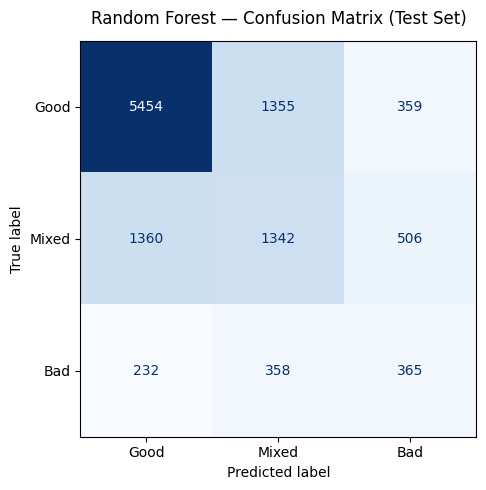
\includegraphics[width=0.55\linewidth]{figures/fig05_rf_cm.png}
  \caption{Row-normalised confusion matrix for the best Random Forest model.}
  \label{fig:rf_cm}
\end{figure}

\subsection{Error flow analysis}

To understand \emph{why} Mixed (F1\,=\,0.43) and Bad (F1\,=\,0.33) are low,
the RF model was refitted with its known best hyperparameters on the full training set
and every test prediction was analysed individually.

\begin{table}[H]
  \centering\small
  \caption{Dominant error patterns in the RF test set.}
  \label{tab:errorflow}
  \begin{tabular}{lrr}
    \toprule
    \textbf{Error type} & \textbf{Count} & \textbf{\% of true class} \\
    \midrule
    Mixed $\to$ Good & 1,360 & 42.4\,\% \\
    Mixed $\to$ Bad  &   505 & 16.6\,\% \\
    Bad $\to$ Mixed  &   358 & 37.5\,\% \\
    Bad $\to$ Good   &   229 & 24.0\,\% \\
    \bottomrule
  \end{tabular}
\end{table}

\textbf{Mixed $\to$ Good} is the dominant failure mode (1,360 cases, 42.4\,\% of all
Mixed games). Mixed games have review ratios between 0.50 and 0.74; many share the same
tags, categories, era, and pricing patterns as Good games. The model has no feature that
encodes the narrow margin between a 0.74 and a 0.76 review ratio.

\textbf{Bad $\to$ Mixed} accounts for 37.5\,\% of Bad errors. Bad is the smallest class
(8.4\,\% of training data); under uncertainty the model defaults toward Mixed.

\subsection{Prediction confidence}

\begin{figure}[H]
  \centering
  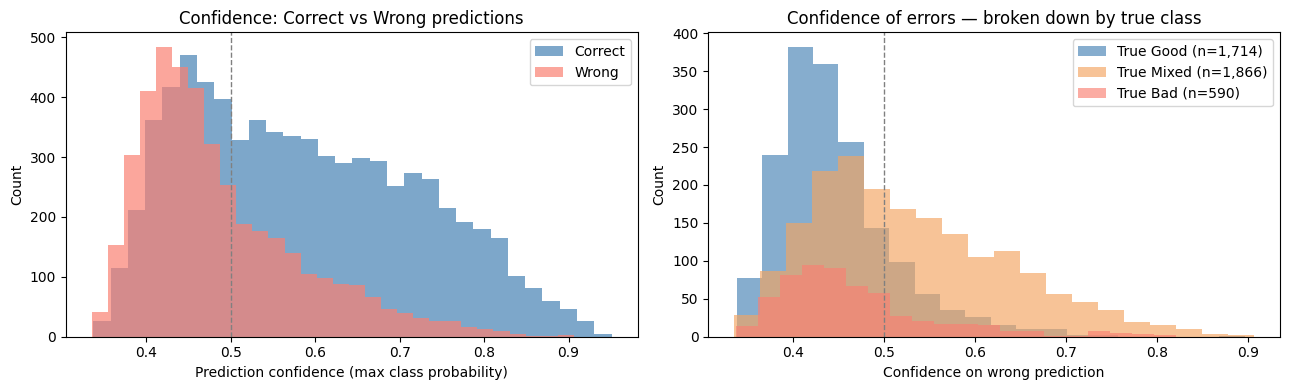
\includegraphics[width=0.80\linewidth]{figures/fig15b_confidence.png}
  \caption{Prediction confidence (max class probability) for correct vs.\ wrong
           test predictions. Correct: median\,=\,0.570; wrong: median\,=\,0.460.}
  \label{fig:confidence}
\end{figure}

Wrong predictions have a median confidence of 0.460, versus 0.570 for correct ones.
The model is systematically uncertain when wrong -- most errors are soft rather than
overconfident misfires. Of 320 high-confidence errors (predicted probability $\geq 0.70$
but wrong), \textbf{243 (75.9\,\%)} are Mixed $\to$ Good, confirming a genuine
feature-space blind spot rather than simple boundary uncertainty.

\subsection{Feature importance and Good vs Mixed separation}

\begin{figure}[H]
  \centering
  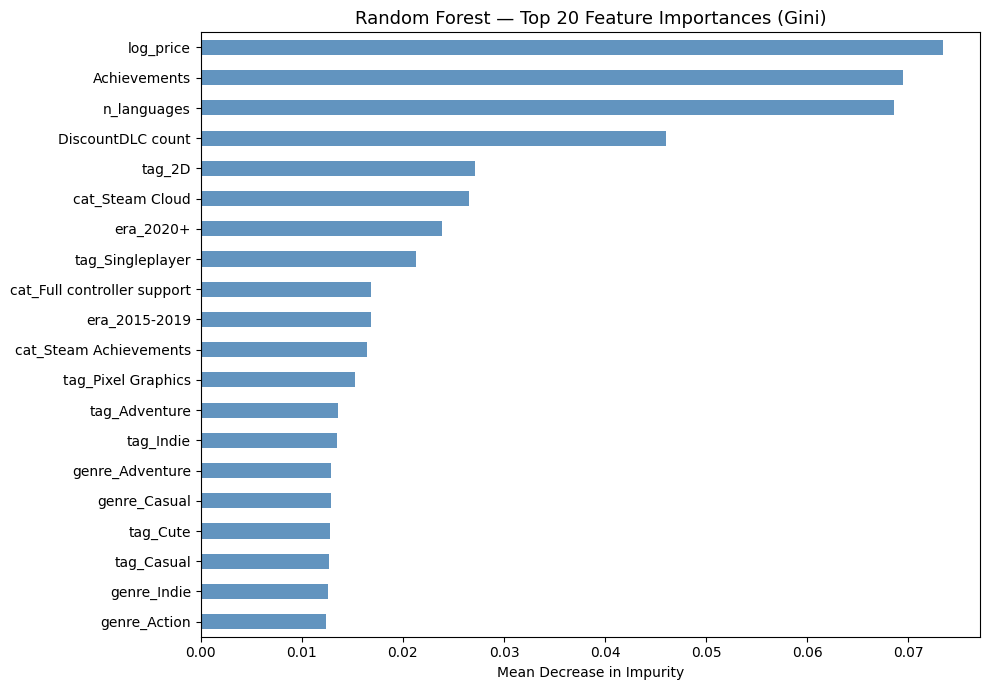
\includegraphics[width=0.70\linewidth]{figures/fig06_rf_importance.png}
  \caption{Top-25 RF feature importances (Gini). Price, achievements, and
           release-era features dominate; individual tag/category indicators
           have lower but collectively significant importance.}
  \label{fig:rf_importance}
\end{figure}

\begin{figure}[H]
  \centering
  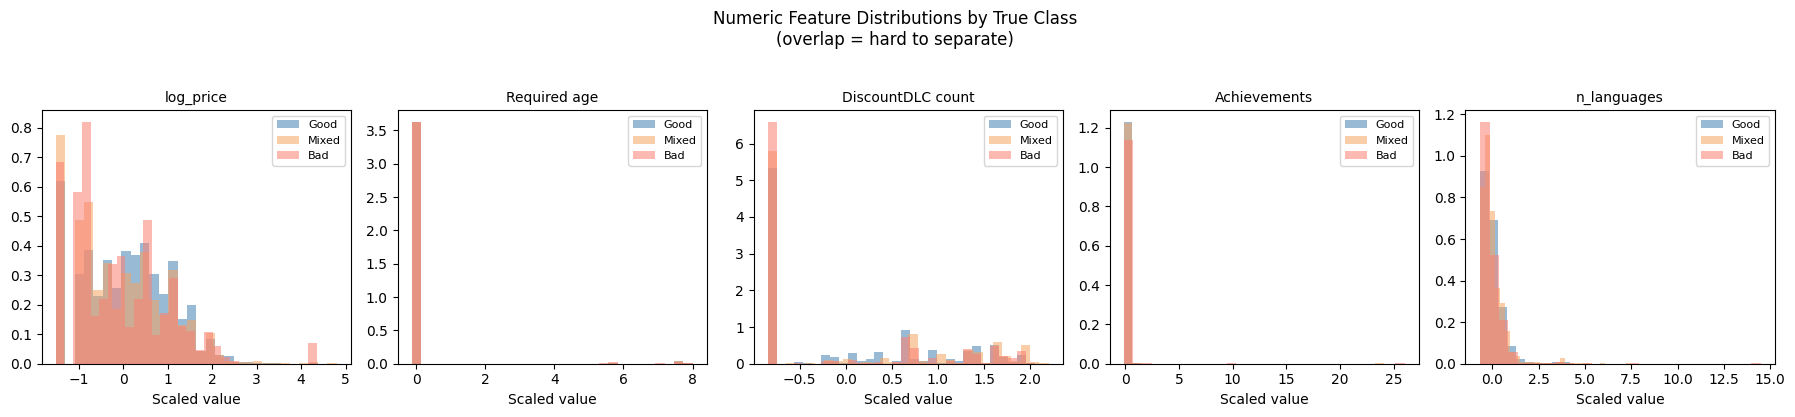
\includegraphics[width=0.88\linewidth]{figures/fig15c_feat_separation.png}
  \caption{Mean feature difference Good $-$ Mixed for the top separating features.
           The strongest signal (\ttf{tag\_2D}, $+$0.172) is modest,
           confirming limited class separation in the feature space.}
  \label{fig:feat_sep}
\end{figure}

Top separating features (mean Good $-$ mean Mixed): \ttf{tag\_2D}\,(+0.172),
\ttf{era\_2020+}\,(+0.159), \ttf{cat\_Steam Cloud}\,(+0.145),
\ttf{era\_2015-2019}\,($-$0.144), \ttf{tag\_Singleplayer}\,(+0.128),
\ttf{cat\_Full controller support}\,(+0.122).
Even the strongest signal (+0.172) is modest, and no single feature cleanly separates
the classes.

\subsection{Threshold-distance analysis}

A supplementary analysis connected each test prediction back to the original
\texttt{review\_ratio} and measured distance to the nearest class boundary.

\begin{itemize}
  \item Mean distance to nearest threshold: 0.1129 (all test), 0.1282 (correct),
        0.0866 (wrong) -- wrong predictions are systematically closer to boundaries.
  \item Severity mix of wrong predictions:
        20\,\% very close to boundary ($<0.05$);
        32\,\% moderately close ($0.05$--$0.15$);
        \textbf{47\,\% far from boundary ($>0.15$)}.
\end{itemize}

Boundary ambiguity explains a significant share of errors but not all of them.
Nearly half of wrong predictions occur for games clearly inside a true class region,
indicating a genuine feature-space limitation rather than only a labelling edge case.

% ============================================================
\section{Feature Engineering Experiment}
\label{sec:fe}

Based on the error analysis, eight derived features were added to the 147-feature dataset
(producing 155 features) and the full RF nested CV was repeated.

\begin{table}[H]
  \centering\small
  \caption{Engineered features and RF results.}
  \label{tab:fe}
  \begin{tabularx}{\linewidth}{llX}
    \toprule
    \textbf{Feature} & \textbf{Type} & \textbf{Rationale} \\
    \midrule
    \ttf{n\_tags}           & count (scaled) & More tags = more discoverable; trends toward Good \\
    \ttf{n\_categories}     & count (scaled) & More Steam categories = release polish proxy \\
    \ttf{n\_genres}         & count (scaled) & Number of genres listed \\
    \ttf{polish\_index}     & sum (scaled)   & Steam Cloud + controller + achievements + Singleplayer + Mac \\
    \ttf{recent\_2d}        & binary         & \ttf{tag\_2D} $\times$ \ttf{era\_2020+} \\
    \ttf{price\_x\_recent}  & interaction    & \ttf{log\_price} $\times$ \ttf{era\_2020+} \\
    \ttf{solo\_only}        & binary         & \ttf{tag\_Singleplayer} $\times$ (1 $-$ \ttf{cat\_Multi-player}) \\
    \ttf{platform\_breadth} & count (scaled) & Windows + Mac + Linux \\
    \bottomrule
  \end{tabularx}
  \vspace{4pt}
  \begin{tabular}{lrrr}
    \toprule
    & \textbf{RF+FE (155 feat.)} & \textbf{Original RF (147 feat.)} & \textbf{Change} \\
    \midrule
    Nested CV Macro F1 & $0.5102 \pm 0.0066$ & $0.5093 \pm 0.0073$ & $+0.0009$ \\
    Test Macro F1      & 0.5093              & \textbf{0.5100}     & $-0.0007$ \\
    \bottomrule
  \end{tabular}
\end{table}

Although 7 of 8 new features ranked in the RF Top~25 by Gini importance
(\ttf{n\_tags} rank~4, \ttf{polish\_index} rank~5, \ttf{price\_x\_recent} rank~7),
performance did not improve.
New count features are \textbf{redundant} with existing binary columns -- the RF
already extracted count-level patterns from the sparse individual tag and category
indicators.
This confirms that the ceiling is set by genuine data ambiguity, not missing
feature engineering.

% ============================================================
\section{Results and Discussion}
\label{sec:results}

\paragraph{Best result.}
Random Forest achieves Test Macro F1 = \textbf{0.5100} -- the highest among all
tested models and +0.0745 over the LR baseline.

\paragraph{Performance ceiling.}
The analysis shows that the task has an inherent ceiling driven by class overlap:
Mixed and Good games share the same metadata patterns, differing only in review ratio.
Current features do not encode execution quality, post-launch support, or community
sentiment -- the signals that actually separate borderline games.

\paragraph{Comparison to related work.}
Prior analyses on the same Kaggle dataset report binary classification accuracy
(Good vs.\ Bad) in the 0.70--0.80 range using simple feature sets \cite{fronkon2024}.
Our multiclass formulation is strictly harder; Macro F1 = 0.51 on three imbalanced
classes corresponds to meaningful discrimination well above a majority-class
baseline (Macro F1 $\approx$ 0.26).

\paragraph{Limitations.}
(1) The safe feature set avoids leakage but excludes the most predictive post-release
signals. (2) Bad remains the hardest class; its recall (0.38) is limited by the small
training sample (8.4\%). (3) Feature engineering added no new information because the
RF already captures count-level patterns from the binary feature space.

\paragraph{Future directions.}
Richer pre-release text features (game description NLP, sentiment of early press),
developer reputation signals, or ensemble stacking could potentially improve Mixed
and Bad F1. A finer threshold exploration around the 0.50/0.75 boundaries may also
reduce the proportion of genuinely borderline cases in the training set.

% ============================================================
\begin{thebibliography}{9}

\bibitem{fronkon2024}
  FronkonGames.
  \textit{Steam Games Dataset.}
  Kaggle, 2024.
  \url{https://www.kaggle.com/fronkongames/steam-games-dataset}

\bibitem{sklearn}
  Pedregosa, F.\ et al.
  \textit{Scikit-learn: Machine Learning in Python.}
  Journal of Machine Learning Research, 12:2825--2830, 2011.

\bibitem{chen2016xgboost}
  Chen, T.\ \& Guestrin, C.
  \textit{XGBoost: A Scalable Tree Boosting System.}
  KDD 2016.

\bibitem{chawla2002smote}
  Chawla, N.\ et al.
  \textit{SMOTE: Synthetic Minority Over-sampling Technique.}
  JAIR, 16:321--357, 2002.

\end{thebibliography}

\end{document}
